\id{IRSTI 31.21.01}{https://doi.org/10.58805/kazutb.v.2.27-884}

\begin{articleheader}
\sectionwithauthors{M.K. Kazankapova, B.T. Yermagambet U.M. Kozhamuratova, Zh.M. Kassenova, A.B. Malgazhdarova, Zh.T. Dauletzhanova, A. Cygan, G.K. Mendaliyev, A.S. Akshekina, F. Tarikhov}{STUDY OF PHYSICOCHEMICAL PROPERTIES OF ADSORBENTS BASED ON POTASSIUM HUMATE AND USE IN HYDROGEN STORAGE}

{\bfseries
\textsuperscript{1,2,3}M.K. Kazankapova\alink{https://orcid.org/0000-0001-9016-3062}\textsuperscript{\envelope },
\textsuperscript{1,2,3}B.T. Yermagambet\alink{https://orcid.org/0000-0003-1556-9526}
\textsuperscript{1,2}U.M. Kozhamuratova\alink{https://orcid.org/0009-0000-7894-5723},
\textsuperscript{1,2}Zh.M. Kassenova\alink{https://orcid.org/0000-0002-9497-7319},
\textsuperscript{1,2}A.B. Malgazhdarova\alink{https://orcid.org/0000-0003-0416-7775},
\textsuperscript{1,3}Zh.T. Dauletzhanova\alink{https://orcid.org/0000-0001-9682-5127},
\textsuperscript{5}A. Cygan\alink{https://orcid.org/0000-0002-1725-2437},
\textsuperscript{1,2}G.K. Mendaliyev\alink{https://orcid.org/0009-0001-5811-4313},
\textsuperscript{1}A.S. Akshekina\alink{https://orcid.org/0009-0006-2181-6019},
\textsuperscript{4}F. Tarikhov\alink{https://orcid.org/0000-0001-6246-4431}
}
\end{articleheader}

\begin{affiliation}
\textsuperscript{1}«Institute of Coal Chemistry and Technology» LLP, Astana, Kazakhstan,

\textsuperscript{2}L.N. Gumilyov Eurasian National University, Astana, Kazakhstan,

\textsuperscript{3}K. Kulazhanov kazakh university of technology and business, Astana, Kazakhstan,

\textsuperscript{4}Nazarbayev University, Astana, Kazakhstan

\textsuperscript{5}ITPE -- Institute Of Technology And Fuel Processing Technology, Zabrze, Poland

\raggedright \textsuperscript{\envelope }Корреспондент-автор: e-mail: maira\_1986@mail.ru, coaltech@bk.ru
\end{affiliation}

This research is based on the investigation of the physicochemical
properties of adsorbents based on potassium humate. During this study,
we evaluated the structure, characteristics, and adsorption capacity of
these materials. Potassium humate served as the main starting material,
and we used a series of high-temperature carbonization and activation
processes to produce the adsorbents we were investigating.

We characterized the surface structure, porosity, and elemental
composition of the resulting adsorbents using techniques such as
cryogenic scanning probe microscopy and scanning electron microscopy
(SEM). We determined the specific surface area of the adsorbents in
terms of surface volume using gas absorption techniques, specifically
the Brunauer-Emmett-Teller (BET) method.

The findings reveal a significant improvement in the porosity and
adsorption properties of activated adsorbents. Most of these materials
have a high specific surface area, which indicates their exceptional
adsorption capacity.

These porous carbonaceous adsorbents, obtained through the methods
described, are well-suited for purifying industrial wastewater and can
act as effective gas adsorbents, including for hydrogen storage. Further
research and experimentation hold promise for even greater improvements.
Based on the results obtained through these methods, potassium
Humate-derived adsorbents emerge as a versatile and technolog\-ically
feasible raw material with wide-ranging applications.

{\bfseries Key words:} adsorbent, potassium humate, adsorption properties,
surface area, activation, storage, hyd\-rogen.

\begin{articleheader}
{\bfseries КАЛИЙ ГУМАТЫ НЕГІЗІНДЕ АЛЫНҒАН АДСОРБЕНТТЕРДІҢ ФИЗИКА-ХИМИЯЛЫҚ ҚАСИЕТТЕРІН ЗЕРТТЕУ ЖӘНЕ СУТЕГІ САҚТАУДА ҚОЛДАНУ}

{\bfseries
\textsuperscript{1,2,3}М.Қ. Қазанқапова\textsuperscript{\envelope },
\textsuperscript{1,2,3}Б.Т. Ермағамбет,
\textsuperscript{1,2}Ұ.М. Қожамұратова,
\textsuperscript{1,2,3}Ж.M. Касенова,
\textsuperscript{1,2}А.Б.~Малғаждарова,
\textsuperscript{1,3}Ж.Т. Даулетжанова,
\textsuperscript{5}А. Цыган
\textsuperscript{1,2}Г.К. Мендалиев,
\textsuperscript{1}Ә.С. Акшекина,
\textsuperscript{4}Ф.~Тарихов
}
\end{articleheader}

\begin{affiliation}
\textsuperscript{1}«Көмір химиясы және технология институты» ЖШС, Астана, Қазақстан,

\textsuperscript{2}Л.Н. Гумилев атындағы Еуразия ұлттық университеті, Астана, Қазақстан,

\textsuperscript{3}Қ.Құлажанов атындағы Қазақ технология және бизнес университеті, Астана, Қазақстан,

\textsuperscript{4}Назарбаев Университеті, Астана, Қазақстан,

\textsuperscript{5}Технологиялар және отын өңдеу технологиясы институты, Забже, Польша,

е-mail: coaltech@bk.ru, maira\_1986@mail.ru
\end{affiliation}

Бұл зерттеу калий гуматы негізіндегі адсорбенттердің физика-химиялық
қасиеттерін зерттеуге негізделген. Осы зерттеу барысында біз осы
материалдардың құрылымын, сипаттамаларын және адсорбциялық қабілетін
бағаладық. Калий гуматы негізгі бастапқы материал ретінде қызмет етті
және біз зерттеген адсорбенттерді алу үшін жоғары температуралы
карбонизация және белсендіру процестерінің сериясын қолдандық.

Біз алынған адсорбенттердің беттік құрылымын, кеуектілігін және
элементтік құрамын криогендік сканерлеу зондтарының микроскопиясы және
сканерлеуші электронды микроскопия (SEM) сияқты әдістерді қолдана отырып
сипаттадық. Біз адсорбенттердің бетінің нақты ауданын газды сіңіру
әдістерін, атап айтқанда Брунауэр-Эмметт-Теллер (BET) әдісін қолдана
отырып, бетінің көлемі бойынша анықтадық.

Нәтижелер белсендірілген адсорбенттердің кеуектілігі мен адсорбциялық
қасиеттерінің айтарлықтай жақсарғанын көрсетеді. Бұл материалдардың
көпшілігінің бетінің жоғары спецификалық ауданы бар, бұл олардың ерекше
адсорбциялық қабілетін көрсетеді.

Сипатталған әдістер арқылы алынған бұл кеуекті көміртекті адсорбенттер
өнеркәсіптік ағынды суларды тазартуға өте қолайлы және тиімді газ
адсорбенттері, соның ішінде сутегін сақтау үшін әрекет ете алады. Әрі
қарайғы зерттеулер мен эксперименттер одан да жақсартуға уәде береді.
Осы әдістер арқылы алынған нәтижелерге сүйене отырып, Калий Гуматынан
алынған адсорбенттер жан-жақты және технологиялық тұрғыдан мүмкін
болатын шикізат ретінде пайда болады.

{\bfseries Түйін сөздер:} адсорбент, калий гуматы, адсорбциялық қасиеттері,
бетінің ауданы, активтенуі, сақталуы, сутегі.

\begin{articleheader}
{\bfseries ИЗУЧЕНИЕ ФИЗИКО-ХИМИЧЕСКИХ СВОЙСТВ АДСОРБЕНТОВ НА ОСНОВЕ ГУМАТА КАЛИЯ И ИСПОЛЬЗОВАНИЕ В ХРАНЕНИИ ВОДОРОДА}

{\bfseries
\textsuperscript{1,2,3}М.Қ. Қазанқапова\textsuperscript{\envelope },
\textsuperscript{1,2,3}Б.Т. Ермағамбет,
\textsuperscript{1,2}Ұ.М. Қожамұратова,
\textsuperscript{1,2,3}Ж.M. Касенова,
\textsuperscript{1,2}А.Б.~Малғаждарова,
\textsuperscript{1,3}Ж.Т. Даулетжанова,
\textsuperscript{5}А. Цыган
\textsuperscript{1,2}Г.К. Мендалиев,
\textsuperscript{1}Ә.С. Акшекина,
\textsuperscript{4}Ф.~Тарихов
}
\end{articleheader}

\begin{affiliation}
\textsuperscript{1}ТОО «Институт химии угля и технологии», Астана, Казахстан,

\textsuperscript{2}Евразийский национальный университет им. Л.Н. Гумилева, Астана, Казахстан,

\textsuperscript{3}Казахский университет технологии и бизнеса имени К. Кулажанова, Астана, Казахстан,

\textsuperscript{4}Назарбаев Университет, Астана, Казахстан,

\textsuperscript{5}Институт технологий и технологий переработки топлива, Забже, Польша,

е-mail: coaltech@bk.ru, maira\_1986@mail.ru
\end{affiliation}

Данное исследование основано на изучении физико-химических свойств
адсорбентов на основе гумата калия. В ходе этого исследования мы оценили
структуру, характеристики и адсорбционную способность этих материалов.
Гумат калия служил основным исходным материалом, и мы использовали ряд
процессов высокотемпературной карбонизации и активации для получения
исследуемых адсорбентов.

Мы охарактеризовали структуру поверхности, пористость и элементный
состав полученных адсорбентов, используя такие методы, как криогенная
сканирующая зондовая микроскопия и сканирующая электронная микроскопия
(SEM). Мы определили удельную поверхность адсорбентов в пересчете на
объем поверхности, используя методы поглощения газа, в частности метод
Брунауэра-Эмметта-Теллера (BET).

Полученные результаты свидетельствуют о значительном улучшении
пористости и адсорбционных свойств активированных адсорбентов.
Большинство из этих материалов имеют высокую удельную поверхность, что
свидетельствует об их исключительной адсорбционной способности.

Эти пористые углеродсодержащие адсорбенты, полученные описанными
способами, хорошо подходят для очистки промышленных сточных вод и могут
выступать в качестве эффективных газовых адсорбентов, в том числе для
хранения водорода. Дальнейшие исследования и эксперименты обещают еще
большие улучшения. Основываясь на результатах, полученных с помощью этих
методов, адсорбенты на основе гумата калия становятся универсальным и
технологически приемлемым сырьем с широким спектром применения.

{\bfseries Ключевые слова:} адсорбент, гумат калия, адсорбционные свойства,
площадь поверхности, активация, хранение, водород.

\begin{multicols}{2}
{\bfseries Introduction.} In light of the global trend towards renewable
energy sources and the mounting environmental concerns, the development
of highly efficient, sustainable, and environmentally friendly materials
assumes paramount importance

{\bfseries The Relevance of the Study.} Natural carbon-based materials,
particularly humic substances such as potassium humate, have garnered
significant attention due to their remarkable chemical reactivity,
abundance, and potential for tailored modification {[}1{]}.

These materials exhibit promising sorption properties, rendering them
suitable for a wide range of applications, including water purification,
gas adsorption, and hydrogen storage. However, a more in-depth
exploration of their activation mechanisms, thermal stability,
structural integrity, and textural characteristics is crucial to fully
appreciate their scientific significance and practical utility.

The purpose of this research is to develop and investigate the
properties of porous sorbents based on potassium humate. Specifically,
we aim to analyze how different activation temperatures affect the
structure, chemical composition, and sorption capacity of these
materials, as well as their potential for hydrogen storage.

In order to accomplish this objective, several tasks were defined:

- To conduct carbonization and activation processes of potassium humate
at various temperatures.

- To characterize the textural properties of the resulting materials
using BET, Raman, and FTIR spectroscopy techniques, as well as
scanning electron microscopy (SEM).

- To determine how heat treatment influences graphitization processes
and the formation of microporous structures.

- To study the hydrogen sorption performance of these materials and
compare it to that of CO₂ and N₂ sorbates.

{\bfseries Scientific breakthrough.} In the course of our research, we
conducted experiments aimed at producing porous carbon that was
activated at elevated temperatures of 800 and 900 degrees Celsius. By
comparing their physicochemical properties, we were able to observe
their characteristics. With an increase in processing temperature, we
observed an enhancement in the quality attributes of the adsorbent and a
corresponding increase in its adsorption capacity. Potassium humate can
be added to the list of environmentally and economically viable
adsorbents.

In the current context of various processes involving man-made waste
contamination, as well as the purification of contaminated wastewaters
and gases, adsorbents play a crucial role as part of composite materials
in the realm of medicine.

In light of these features and advantages, research into the development
of porous materials based on humic substances is gaining momentum. The
structure of potassium humate, the primary component of adsorbents,
exhibits remarkable complexity. Due to the presence of diverse
functional groups, it demonstrates rapid reactivity with a wide range of
metals and simple substances, indicating its high chemical activity
{[}2,3{]}.

Within this functional structure, carboxyl, phenolic, and hydroxyl
groups can be identified {[}4{]}. Studies have demonstrated that
modifications to humates, such as carbonization and activation,
significantly enhance their specific surface area, porosity, and
selective adsorption capabilities.. The activation of humates through
physicochemical methods, such as thermal treatment, exposure to water
vapor, carbon dioxide or chemical reagents, can result in the formation
of a highly porous structure with exceptional adsorption capacity.
Potassium humate, a specific type of humic substance, holds significant
potential in agriculture due to its capacity to enhance the physical and
chemical characteristics of soil, promote root system development, and
bolster plant resilience against abiotic stressors. The utilization of
potassium humate fosters more efficient nutrient absorption, allowing
for a reduction in mineral fertilizer application without compromising
crop yield {[}5{]}. Moreover, the use of granular forms of potassium
humate has been demonstrated to enhance soil water-holding capacity and
stimulate microbiological processes.. Humic substances (HS), which are
formed through the process of humification and carbonization of natural
organic materials such as lignite, brown coal, Leonardite, and peat,
play a crucial role in soil ecosystems {[}6,7{]}. They constitute the
dominant component of soil organic matter, accounting for 60--80\% of
the total organic matter and 50--80\% of dissolved organic matter in
water, with a concentration of 25\% in groundwater.

These substances contribute to soil water retention, regulate the
formation of soil aggregates, facilitate carbon sequestration, and
impact the dynamics of soil microorganisms. However, extracting HS from
natural organic materials presents significant challenges due to their
tendency to bind with humins, polyvalent cations, and heavy metals,
rendering them insoluble and less accessible for agricultural use
{[}8{]}.

Research has shown that materials based on humates effectively remove
heavy metals and organic contaminants from aqueous solutions, while
other studies have explored the use of humic sorbents in gas separation
and air purification processes.. The study conducted by {[}9{]}
highlights the advantages of humic sorbents, such as their lower cost
and upgradeability compared to activated carbon. Furthermore, research
{[}10{]} has explored various methods for activating humic substances,
including treatments with CO\textsubscript{2}, steam, and ozone,
allowing for precise control over the structure of the material
{[}11{]}. However, optimizing activation conditions and enhancing
mechanical strength remains a challenging task.

A number of investigations have demonstrated that adsorbents based on
potassium humate can effectively eliminate heavy metals, organic
contaminants, petroleum products, and other toxic substances from
aqueous solutions, as reported in {[}12{]} and {[}13{]}. In the study
{[}14{]}, it was demonstrated that treating humates in a
CO\textsubscript{2} atmosphere increases their surface area and forms a
mesoporous structure, enhancing their capacity to absorb metal ions such
as Pb\textsuperscript{2+} and Cd\textsuperscript{2+}. Further
investigations suggest the potential application of humate-laden
adsorbents for capturing gases such as CO₂ and H₂C, thereby paving the
way for their utilization in gas separation processes and air
purification procedures {[}15{]}. Moreover, adsorbents based on humic
substances exhibit similar advantages to activated carbon when compared
to conventional sorbents, owing to their affordability, renewable
nature, and capacity for chemical modification of their structure to
enhance sorption performance {[}16{]}.

Nevertheless, there remain unresolved challenges related to optimizing
activation methods, enhancing the mechanical durability of the resulting
materials, and investigating their regenerative capabilities {[}17{]}.
In this study, we delve into the physicochemical characteristics of
adsorbents derived from potassium humate, examining their structure,
porosity, and sorption efficacy.

{\bfseries Materials and methods.} In order to conduct this research, we
employed state-of-the-art laboratory instruments and equipment,
including a quartz reactor, a rotary tube furnace, a gas chromatograph,
a shaker-incubator, and a spectrophotometer, as well as a microscope
equipped with a pH meter, a centrifuge, an ultrasonic bath, and an
electron quantum scanning device.

The process of carbonization and activation to produce potassium
humate-based carbon adsorbents occurred under laboratory conditions in a
nitrogen-filled environment at a temperature of 500 degrees Celsius.
Carbonization serves the purpose of eliminating volatile components and
establishing a porous structure in the material. For activation, water
vapor was employed, which facilitated the development of a microporous
framework.

Various methods were employed to investigate the physicochemical
characteristics of the resulting adsorbents. X-ray diffraction analysis
was conducted using an X-ray diffractometer equipped with Cu Ka
radiation, spanning a range from 5 to 90 degrees of diffraction angle,
to examine the phase composition and crystal structure.. The analysis of
infrared (IR) spectra was conducted in the laboratories of «Nazarbayev
University» using a Nicolet iS10 Fourier transform infrared (FTIR)
spectrometer. To evaluate the porous structure and specific surface area
of the materials, gas adsorption was employed using the
Brunauer-Emmett-Teller (BET) method. Scanning electron microscopy (SEM)
allowed us to investigate the morphology and surface structure of the
adsorbents, while the adsorption properties were explored using methyl
orange, enabling the determination of the materials'{https://doi.org/10.58805/kazutb.v.2.27-884}
activity in solutions containing organic pollutants.

The elemental composition of the materials was analysed using a Quanta
3D 200i scanning electron microscope equipped with an energy dispersive
X-ray analyser (EDAX detector). Additionally, the pH levels of aqueous
solutions containing the adsorbents were measured using a pH meter,
providing insights into their acid--base properties. All experiments
were conducted multiple times.

{\bfseries Results and discussion.} The gas chromatographic analysis
revealed the primary composition of gases emitted during the processes
of carbonization and activation of potassium humate.

At a temperature of 800°C, the concentration of oxygen was 38.033\%,
hydrogen - 27.612\%, carbon dioxide - 6.966\%, nitrogen - 1.532\%, and
methane - 9.767\%.

During pyrolysis at a temperature of 900°C, oxygen concentration
decreased to 7.39\%, while hydrogen increased to 17.68\%. The
concentration of carbon dioxide remained relatively stable at 5.58\%.
Nitrogen concentration rose to 69.35\%, indicating a significant
increase in its proportion. Carbon monoxide was also detected in the gas
mixture.

Detailed information on the composition of gases and material balance
during carbon activation is provided in Tables 1-4, which showcase the
elemental composition of the released gases.

At the initial stage of the thermal processing of potassium humate,
there is a process of dehydration, accompanied by the release of water
and volatile compounds with a low molecular weight. As the temperature
continues to rise, the decomposition of carboxyl, phenolic, and other
oxygen-containing functional groups commences, resulting in the emission
of CO\textsubscript{2}, CO, and a minor amount of volatile organic
compounds.
\end{multicols}

\tcap{Table 1 - Material balance of potassium humate activation at 800℃}
\begin{longtblr}[
  label = none,
  entry = none,
]{
  cells = {c},
  cell{2}{1} = {r=3}{},
  cell{5}{1} = {r=4}{},
  vlines,
  hline{1-2,5,9} = {-}{},
  hline{3-4,6-8} = {2-4}{},
}
 & \textbf{Name} & \textbf{Massa, g} & \textbf{Compound, \%}\\
Original & Potassium humate & 270.0 & 90.0\\
 & Water & 30.00 & 10.00\\
 & Total & 300.00 & 100.00\\
 Product & Solid residue (adsorbent) & 172.00 & 57.30\\
 & Generator gas & 97.40 & 32.50\\
 & Liquid product (water + resin) & 30.60 & 10.20\\
 & Total & 300.00 & 100.0
\end{longtblr}

\tcap{Table 2 - Material balance of potassium humate activation at 900℃}
\begin{longtblr}[
  label = none,
  entry = none,
]{
  cells = {c},
  cell{2}{1} = {r=3}{},
  cell{5}{1} = {r=4}{},
  vlines,
  hline{1-2,5,9} = {-}{},
  hline{3-4,6-8} = {2-4}{},
}
& \textbf{Name} & \textbf{Massa, g} & \textbf{Compound, \%}\\
Original & Potassium humate & 200.00 & 66.67\\
 & Water & 100.00 & 33.33\\
 & Total & 300.00 & 100.00\\
 Product & Solid residue (adsorbent) & 68.40 & 22.80\\
 & Generator gas & 201.66 & 67.22\\
 & Liquid product (water + resin) & 29.94 & 9.98\\
 & Total & 300.00 & 100.00
\end{longtblr}

\tcap{Table 3 - Gas composition of carbonization and humate activation at 800℃}
\begin{longtblr}[
  label = none,
  entry = none,
]{
  cells = {c},
  cell{1}{1} = {r=2}{},
  cell{1}{2} = {r=2}{},
  cell{1}{3} = {c=5}{},
  cell{3}{1} = {r=5}{},
  cell{8}{1} = {r=2}{},
  vlines,
  hline{1,3,8,10} = {-}{},
  hline{2} = {3-7}{},
  hline{4-7,9} = {2-7}{},
}
\textbf{Process} & \textbf{Т, С°} & \textbf{Gas composit vol., \%} &  &  &  & \\
 &  & О\tsb{2} & H\tsb{2} & CO\tsb{2} & N\tsb{2} & CO\\
Carbonization & 200 & 53.94 & 0.07 & - & 46.05 & -\\
 & 300 & 37.52 & 0.71 & 9.45 & 22.34 & 27.83\\
 & 400 & 50.99 & 5.98 & 15.39 & 29.69 & -\\
 & 500 & 30.17 & 6.73 & 19.43 & 45.77 & -\\
 & 600 & 28.03 & 17.61 & 6.96 & 47.53 & -\\
Activation & 700 & 22.31 & 19.56 & 7.89 & 42.31 & -\\
 & 800 & 19.14 & 16.37 & 7.93 & 57.25 & -
\end{longtblr}

\tcap{Table 4 - Gas composition of carbonization and humate activation at 900℃}
\begin{longtblr}[
  label = none,
  entry = none,
]{
  cells = {c},
  cell{1}{1} = {r=2}{},
  cell{1}{2} = {r=2}{},
  cell{1}{3} = {c=4}{},
  cell{3}{1} = {r=5}{},
  cell{8}{1} = {r=3}{},
  vlines,
  hline{1,3,8,11} = {-}{},
  hline{2} = {3-6}{},
  hline{4-7,9-10} = {2-6}{},
}
\textbf{Process} & \textbf{Т, С°} & \textbf{Gas composit vol., \%} &  &  & \\
 &  & \textbf{О\tsb{2}} & \textbf{H\tsb{2}} & \textbf{CO\tsb{2}} & \textbf{N\tsb{2}}\\
Carbonization & 200 & 8.79 & 2.18 & - & 89.03\\
 & 300 & 12.62 & 31.07 & 0.40 & 55.91\\
 & 400 & 10.89 & 8.16 & 0.47 & 80.48\\
 & 500 & 8.29 & 9.91 & 4.07 & 77.73\\
 & 600 & 5.68 & 10.44 & 5.24 & 78.64\\
Activation & 700 & 2.96 & 4.93 & 5.89 & 86.31\\
 & 800 & 10.42 & 13.12 & 4.21 & 72.25\\
 & 900 & 7.39 & 17.68 & 5.58 & 69.35
\end{longtblr}

\tcap{Table 5 - Elemental composition of the initial and activated samples}
\begin{longtblr}[
  label = none,
  entry = none,
]{
  width = \linewidth,
  colspec = {Q[354]Q[71]Q[71]Q[60]Q[62]Q[60]Q[60]Q[58]Q[71]Q[58]},
  cells = {c},
  cell{1}{1} = {r=2}{},
  cell{1}{2} = {c=9}{},
  vlines,
  hline{1,3-6} = {-}{},
  hline{2} = {2-10}{},
}
\textbf{Name} & \textbf{Content	of elements, wt. \%} &  &  &  &  &  &  &  & \\
 & \textbf{C} & \textbf{O} & \textbf{Na} & \textbf{Mg} & \textbf{Al} & \textbf{Si} & \textbf{S} & \textbf{K} & \textbf{Fe}\\
Initial potassium humate & 42.94 & 26.16 & 0.62 & 0.21 & 1.27 & 0.48 & 0.26 & 25.92 & 2.14\\
Activated potassium humate 800℃ & 51.06 & 27.69 & 0.81 & 0.21 & 0.95 & 0.37 & 0.24 & 16.71 & 1.96\\
Activated potassium humate 900℃ & 29.45 & 31.22 & 3.86 & 0.08 & 0.56 & 0.25 & 0.18 & 34.07 & 0.33
\end{longtblr}

\begin{figure}[H]
    \centering
    \begin{subfigure}[t]{0.45\textwidth}
        \centering
        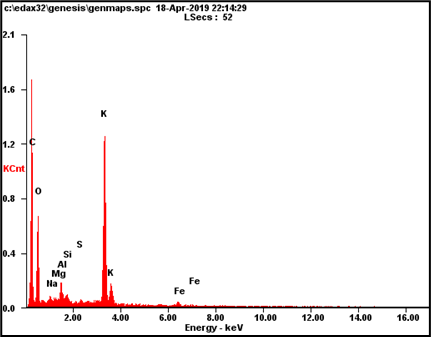
\includegraphics[height=5.1cm]{media/chem2/image87}
        \caption*{a}
    \end{subfigure}
    \begin{subfigure}[t]{0.45\textwidth}
        \centering
        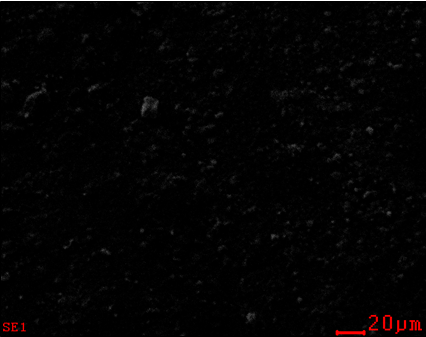
\includegraphics[height=5.1cm]{media/chem2/image88}
        \caption*{b}
    \end{subfigure}
    
    \begin{subfigure}[t]{0.45\textwidth}
        \centering
        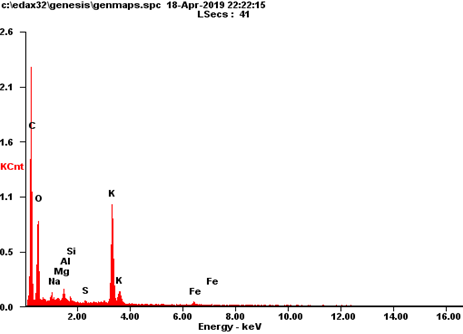
\includegraphics[height=5.1cm]{media/chem2/image89}
        \caption*{c}
    \end{subfigure}
    \begin{subfigure}[t]{0.45\textwidth}
        \centering
        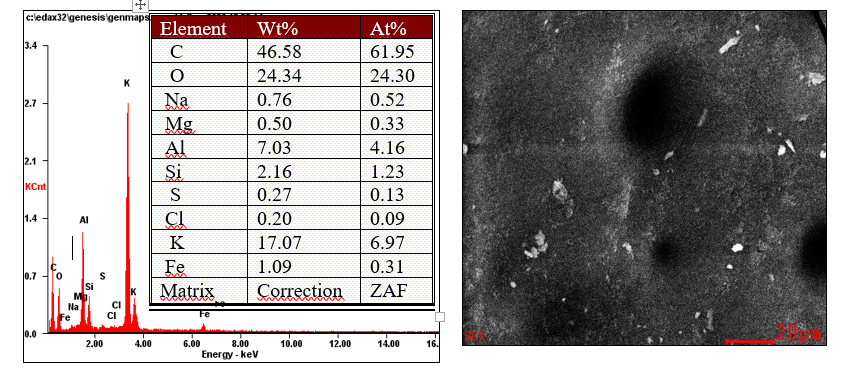
\includegraphics[height=5.1cm]{media/chem2/image90}
        \caption*{d}
    \end{subfigure}
    
    \begin{subfigure}[t]{0.45\textwidth}
        \centering
        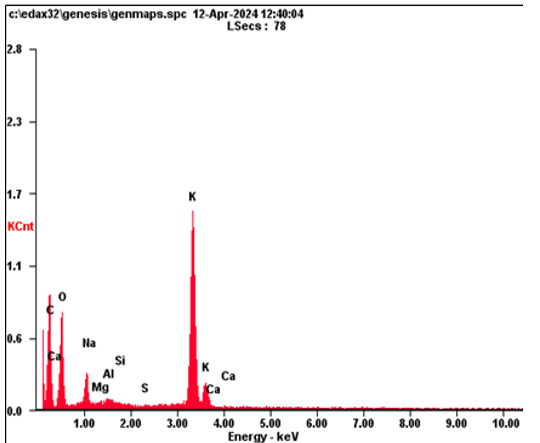
\includegraphics[height=5.1cm]{media/chem2/image91}
        \caption*{e}
    \end{subfigure}
    \begin{subfigure}[t]{0.45\textwidth}
        \centering
        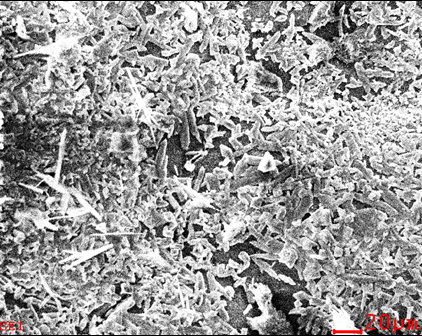
\includegraphics[height=5.1cm]{media/chem2/image92}
        \caption*{f}
    \end{subfigure}
    \caption*{{\bfseries Fig.1 - Elemental composition of samples (a, b -- initial potassium humate; c, d - activated potassium humate 800℃; e, f - activated potassium humate 900℃)}}
\end{figure}

\begin{multicols}{2}
With an increase in temperature, aromatic and aliphatic components of
the humate structure undergo destruction, leading to the formation of
resinous intermediate products. These substances can participate in
structural reorganization processes, contributing to the creation of
more thermodynamically stable carbon systems.

At higher temperatures ranging from 600 to 700 degrees Celsius,
carbonization and condensation reactions become predominant, resulting
in the production of a carbonaceous residue with a highly porous
structure.. The presence of potassium in a given environment promotes
the catalytic breakdown of organic constituents, thereby facilitating
the creation of microporous carbon materials. This process is of utmost
significance in the manufacturing of activated carbon and sorbent
materials. The findings regarding the elemental composition of the
examined samples are detailed in Table 5 and illustrated in Figure 1.

Based on the table data, the original potassium humate contains 42.94\%
C, 26.16\% O\textsubscript{2}, 0.62\% Na, 0.21\% Mg, 1.27\% Al, 0.48\%
Si, 0.26\% S, 25.92\% K and 2.14\% Fe.

Following activation at a temperature of 800 degrees Celsius, the carbon
content rises to 51.06 percent, oxygen to 27.69 percent, sodium to 0.81
percent, while magnesium remains unchanged at 0.21 percent. Aluminium
decreases to 0.95 percent, silicon to 0.37 percent, sulphur to 0.24
percent, potassium content declines to 16.71 percent, and iron to 1.96
percent.

Upon activation at 900 degrees Celsius, the carbon content of the
material significantly decreases to a level of 29.45 percent, while the
oxygen content rises to 31.22 percent. The sodium concentration
diminishes to 3.86 percent, magnesium to 0.08 percent, aluminum to 0.56
percent, silicon to 0.25 percent, and sulfur to 0.18 percent.
Conversely, the potassium content rises to a value of 34.07 percent,
while iron content decreases to 0.33 percent.

The presence of potassium within the humate framework serves as a
catalyst, activating thermal decomposition reactions and promoting the
expansion of the overall porous structure.. At temperatures exceeding
700 degrees Celsius, the process of active micropore formation
commences, resulting in a substantial increase in the specific surface
area of the material. The precise pore structure is contingent upon the
conditions of heat treatment: at lower temperatures, mesopores dominate,
providing exceptional sorption capacity for larger molecules, while
high-temperature activation between 900 and 1000 degrees Celsius leads
to the formation of well-developed micropores, further enhancing the
specific surface area and rendering the material highly effective as a
sorbent for both gases and smaller molecules.

The micrographs of both the original and activated samples can be seen
in Figure 2. Upon analyzing the morphology of these adsorbents, it
became evident that the dimensions of the particles exhibit a
non-homogeneous structure. The adsorbent treated with potassium humate
and subsequently dried at 900 degrees Celsius exhibited dimensions
ranging from 295.4 to 548.2 nanometers, while the adsorbent treated with
the same potassium humate but at 800 degrees Celsius had dimensions
ranging between 41.2 and 71.1 nanometers.

As seen in Figure 2, the formation of carbon nanotubes is observed at
800\,°C, where at 900\,°C, other carbon materials are predominantly
formed. The pores in the structure of potassium humate are formed as a
result of heat treatment and chemical activation, which helps to
increase the specific surface area and improve the adsorption properties
of the material. These pores have different sizes, which allows
potassium humate to effectively interact with gases and liquids.

The presence of some large particles and large pores is also observed,
which may indicate the initial stage of structural changes in the
material. The structure of potassium humate appears to be quite loose
and porous, which determines its high activity and potential for use in
various applications, such as adsorption or catalysis.
FTIR is an effective analytical method used to study the chemical
structure and composition of potassium humate. This material, a salt of
humic acids obtained as a result of the decomposition of organic
substances in soil and peat, undergoes significant structural changes
when exposed to high-temperature activation. A comparison of the spectra
obtained at 800 ℃ and 900 °C shows the evolution of functional groups
during heat treatment.

Both spectra exhibit characteristic absorption bands associated with
humic substances. The wide band around 3438-3445 cm\textsuperscript{--1}
corresponds to the stretching fluctuations of hydroxyl (O-H), which
indicates the presence of water, alcohol, or phenolic groups. The range
of \textasciitilde1630 cm\textsuperscript{-1} reflects fluctuations in
carbonyl (C=O) and unsaturated C=C bonds, usually extending from
aromatic rings. The 1404 cm\textsuperscript{--1} peak is caused by
bending vibrations of C--h and deformation of O-H in humus structures.
Ranges of 1010-1125 cm\textsuperscript{-1} show fluctuations in the
stretching of C-O, which suggests the presence of alcohol or phenolic
functions important for metal bonding. The area of approximately 830
cm\textsuperscript{-1} and 700 cm\textsuperscript{-1} confirms the
structures of aromatic rings, bending beyond the C--H plane. The ranges
of \textasciitilde2610 and 2950 cm\textsuperscript{-1} are associated
with asymmetric and symmetrical C--H stretching fluctuations, usually
observed in aromatic and aliphatic groups (Table 6).
\end{multicols}

\begin{figure}[H]
    \centering
    \begin{subfigure}[t]{0.45\textwidth}
        \centering
        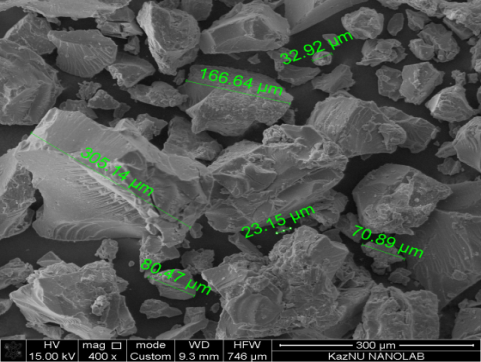
\includegraphics[height=5.5cm]{media/chem2/image93}
        \caption*{a}
    \end{subfigure}
    \begin{subfigure}[t]{0.45\textwidth}
        \centering
        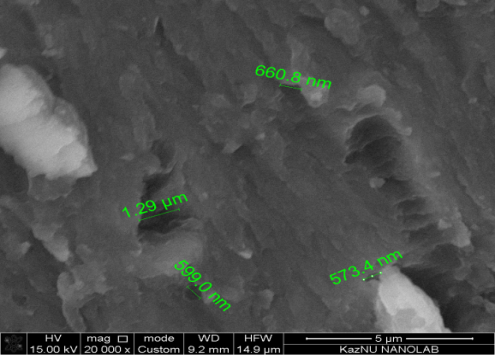
\includegraphics[height=5.5cm]{media/chem2/image94}
        \caption*{b}
    \end{subfigure}
    
    \begin{subfigure}[t]{0.45\textwidth}
        \centering
        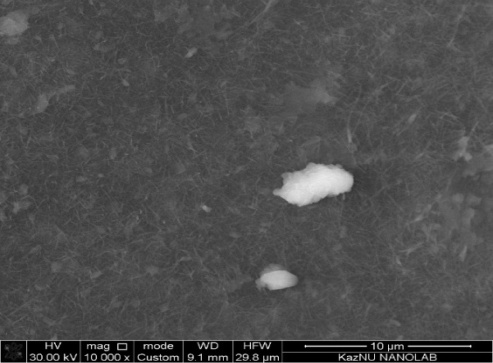
\includegraphics[height=5.5cm]{media/chem2/image95}
        \caption*{c}
    \end{subfigure}
    \begin{subfigure}[t]{0.45\textwidth}
        \centering
        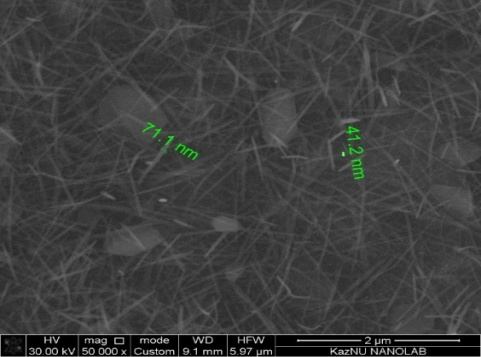
\includegraphics[height=5.5cm]{media/chem2/image96}
        \caption*{d}
    \end{subfigure}
    \begin{subfigure}[t]{0.45\textwidth}
        \centering
        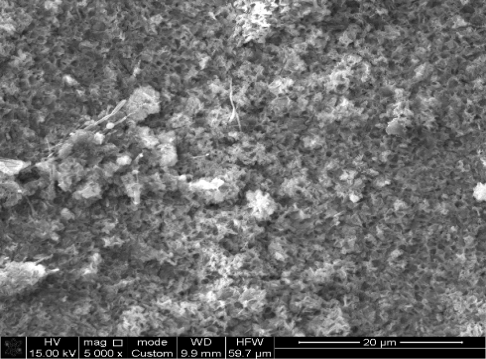
\includegraphics[height=5.5cm]{media/chem2/image97}
        \caption*{e}
    \end{subfigure}
    \begin{subfigure}[t]{0.45\textwidth}
        \centering
        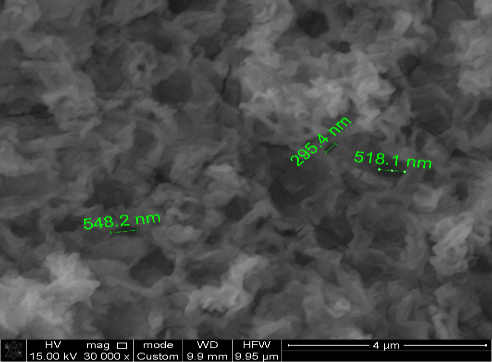
\includegraphics[height=5.5cm]{media/chem2/image98}
        \caption*{f}
    \end{subfigure}
    \caption*{{\bfseries Fig.2 - SEM images of samples (a, b - initial potassium humate; c, d - activated potassium humate 800℃; e, f - activated potassium humate 900℃)}}
\end{figure}

\begin{multicols}{2}
Figure 3 shows the IR spectra of potassium Humate activated at different
temperatures-800°C and 900°C, showing changes in the composition of
functional groups as a result of heat treatment.

An increase in the activation temperature from 800°C to 900°C leads to
small but significant edits in the FTIR absorption bands, especially in
the carbonyl and C--O regions, which indicates continuous decomposition
or rearrangement of organic functional groups. The loss of the 510
cm\textsuperscript{⁻1} band at 900°C means a possible rupture of
metal-organic interactions or complexes. Despite the thermal stress, the
aromatic structures remain quite unchanged, which is expressed in the
preservation of peaks below about 830 cm\textsuperscript{⁻1} and 700
cm\textsuperscript{⁻1}. In general, the Humate activated at 900°C is
structurally stabilized and enriched with aromatic content, the volatile
and unstable functional groups are reduced. The results of Raman
spectroscopy of potassium Humate activated at 800 °C indicate the
presence of peaks D (1359 cm\textsuperscript{-1}) and G (1575.8
cm\textsuperscript{-1}). The degree of graphitization for a given sample
is 22.13\%, which is determined using spectroscopic methods such as
Gaussian decay of the spectrum. The intensity ratio of peaks D and G is
I//I = = 0.86, and the obrat inverse ratio I / / I calculated by the
Gaussian method is 1.15.
\end{multicols}

\begin{figure}[H]
    \centering
    \begin{subfigure}[t]{0.45\textwidth}
        \centering
        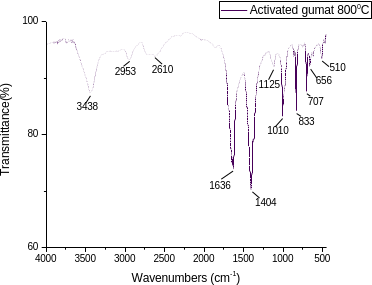
\includegraphics[width=\textwidth]{media/chem2/image99}
        \caption*{a}
    \end{subfigure}
    \begin{subfigure}[t]{0.45\textwidth}
        \centering
        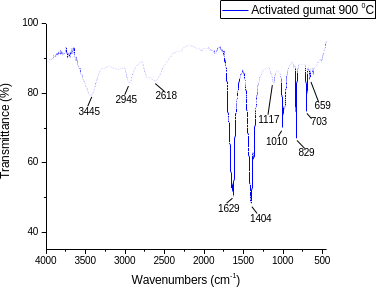
\includegraphics[width=\textwidth]{media/chem2/image100}
        \caption*{b}
    \end{subfigure}
    \caption*{Fig.3 - IR spectra of potassium humate at 800°C (a) and 900°C (b)}
\end{figure}

\begin{multicols}{2}
With an increase in the activation temperature to 900°C, the structure
of the carbon material undergoes significant changes. In this sample,
the degree of graphitization decreases compared to potassium Humate
activated at 800°C, which may be due to the redistribution of carbon
phases and changes in the structure defect. As a result, its adsorption
properties and catalytic activity can be affected.

Thus, heat treatment at different temperatures significantly affects the
degree of graphitalization of potassium Humate, as well as its
structural and functional characteristics. An increase in the activation
temperature leads to an increase in the defect of the carbon material,
which is confirmed by a change in spectral characteristics.
\end{multicols}

\tcap{Table 6 - Key Differences at 800\,°C and 900\,°C Spectr}
\begin{longtblr}[
  label = none,
  entry = none,
]{
  width = \linewidth,
  colspec = {Q[140]Q[125]Q[125]Q[546]},
  cells = {c},
  hlines,
  vlines,
}
\textbf{Spectral			Region} & \textbf{800 °C} & \textbf{900 °C} & \textbf{Interpretation}\\
O–H
			Stretching & 3438			cm\textsuperscript{-1} & 3443			cm\textsuperscript{-1} & Slight
			shift, possibly due to changes in hydrogen bonding or moisture
			content.\\
C=O
			/ C=Stretch C & 1635			cm\textsuperscript{-1} & 1626			cm\textsuperscript{-1} & A
			downward shift indicates the weakening or rearrangement of
			carbonyl/aromatic groups.\\
C–O
			Stretch & 1125			-			1010 cm\textsuperscript{-1} & 1118			-			1010 cm\textsuperscript{-1} & A
			slight decrease in wavenumber may be due to the breaking or
			structural rearrangement of ether/phenolic bonds.\\
C-H
			Aromatic Bend & 833
			cm⁻¹ & 827			cm\textsuperscript{-1} & A
			very small shift indicates a stable aromatic character.\\
C–H
			Out-of-Plane Bend & 706			-			656 cm\textsuperscript{-1} & 702			-			659 cm\textsuperscript{-1} & Minimal
			changes confirm the preservation of aromatic ring systems.\\
Low
			Frequency Vibration & 510			cm\textsuperscript{-1} & Abs & A
			disappearance may indicate the decomposition of organometallic
			complexes at 900°C.\\
Asymmetric
			Stretch C-H & 2611			cm\textsuperscript{-1} & 2614			cm\textsuperscript{-1} & A
			slight shift towards magnification indicates changes in the local
			environment of aromatic/aliphatic C–H bonds.\\
Symmetric
			Stretch C-H & 2952			cm\textsuperscript{-1} & 2945			cm\textsuperscript{-1} & A
			slight decrease towards magnification indicates a slight
			structural rearrangement of organic structures.
\end{longtblr}

\begin{figure}[H]
    \centering
    \begin{subfigure}[t]{0.45\textwidth}
        \centering
        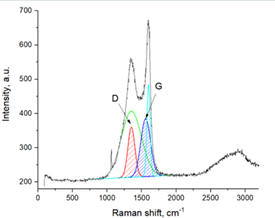
\includegraphics[height=5cm]{media/chem2/image101}
        \caption*{a}
    \end{subfigure}
    \begin{subfigure}[t]{0.45\textwidth}
        \centering
        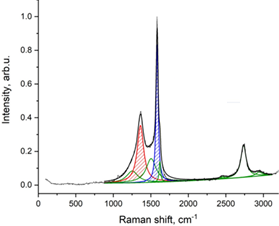
\includegraphics[height=5cm]{media/chem2/image102}
        \caption*{b}
    \end{subfigure}
    \caption*{Fig.4 - Raman spectr of activated potassium humate at 800℃ (a) and at 900℃ (b)}
\end{figure}

\begin{multicols}{2}
Potassium Humate interesting sorption properties that can be studied by
adsorbing nitrogen. Nitrogen adsorption isotherms for potassium Humate
show characteristic features of a microporous structure, which is
confirmed by the fact that isotherms belong to type I. That is,
potassium Humate has a high surface area, mainly consisting of
micropores with a diameter of no more than a few nitrogen molecules. The
process of nitrogen adsorption in potassium Humate is accompanied by
saturation of the micropores of the material with nitrogen molecules,
which leads to the formation of a horizontal site in the isotherm, where
adsorption occurs at low pressure values. This suggests that the
material is capable of effectively capturing gas molecules in
microporous space. With increasing pressure, nitrogen fills the existing
pores, but at higher pressure values, adsorption reaches saturation,
which is confirmed by the presence of a horizontal site in the isotherm.
Potassium Humate also exhibits a type IV hysteresis cycle, which may
indicate the presence of slit-like pores in its structure, typical of
organic materials with a multilayer porous mesh. This allows potassium
Humate to interact effectively with various gases, including nitrogen,
making it useful in a variety of sorption and catalytic applications.
\end{multicols}

\begin{figure}[H]
	\centering
	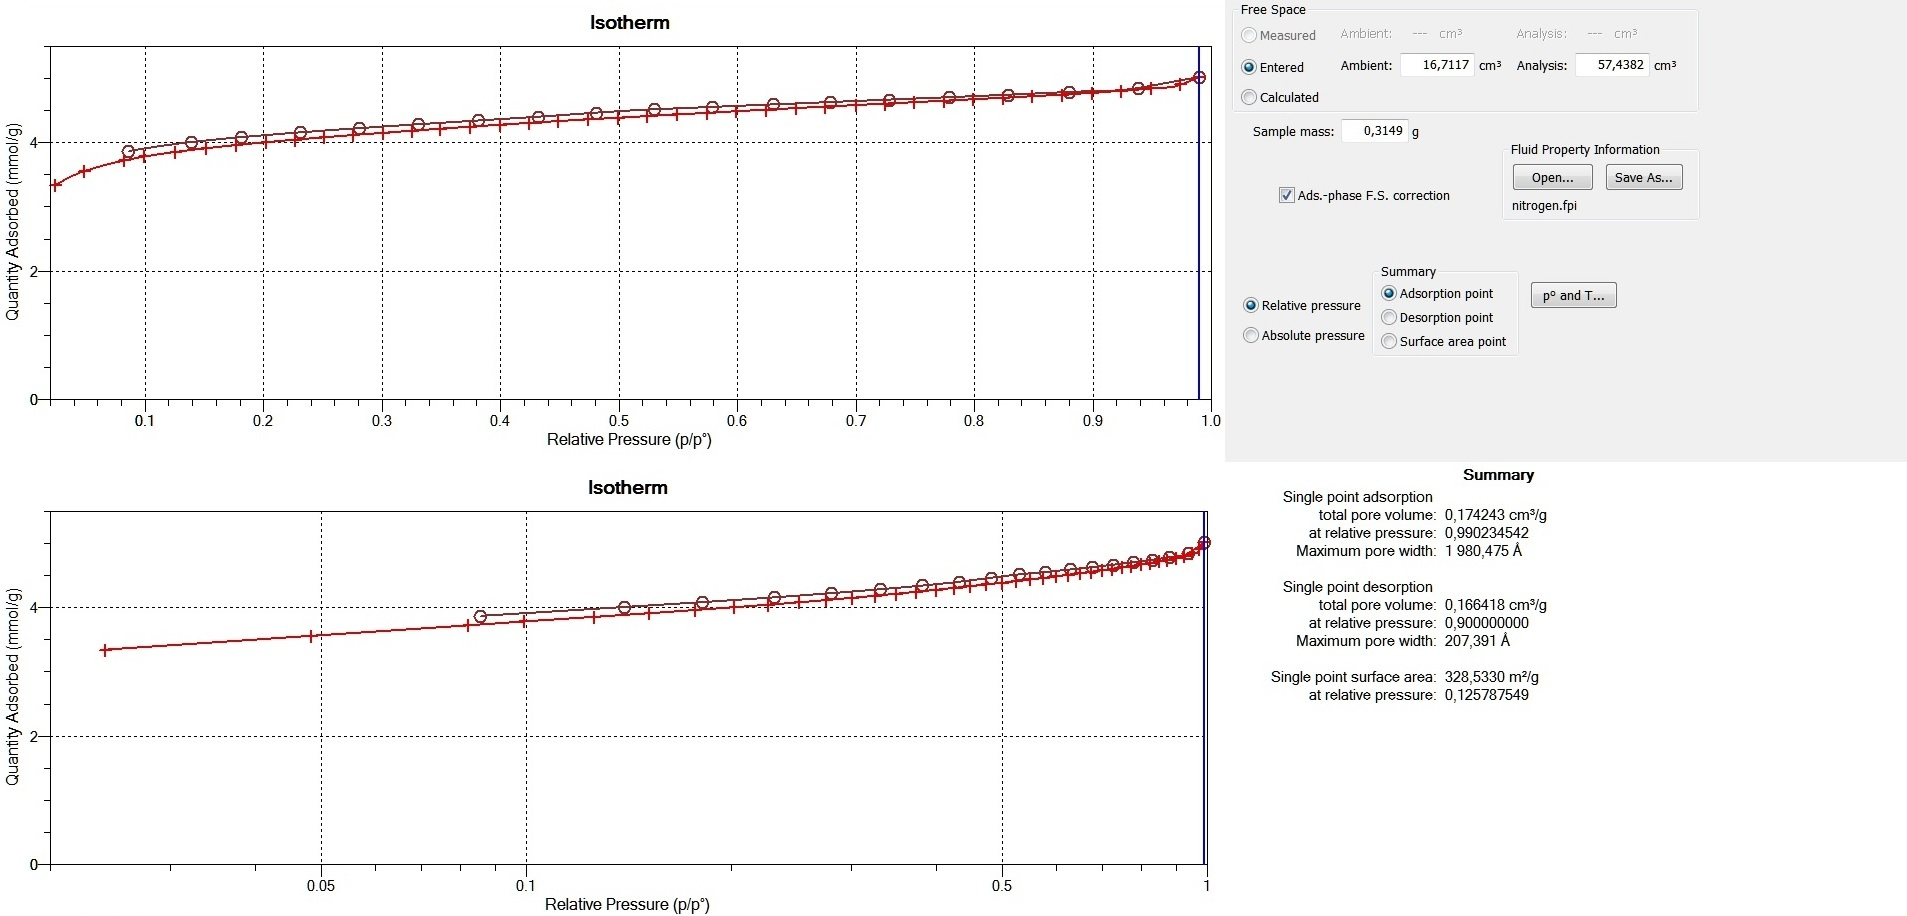
\includegraphics[width=0.85\textwidth]{media/chem2/image103}
	\caption*{a}
	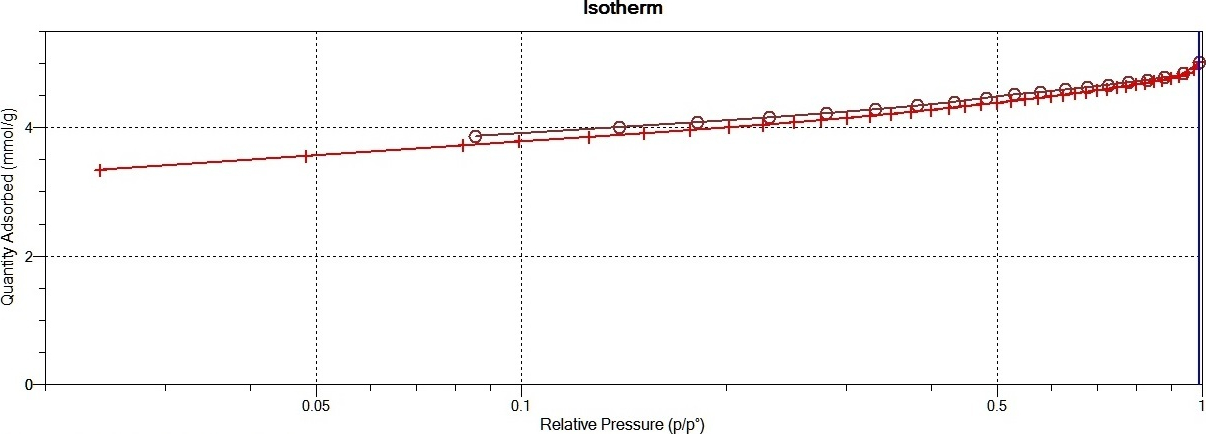
\includegraphics[width=0.85\textwidth]{media/chem2/image103.1}
	\caption*{b}
	\caption*{Fig.5 - Adsorption of activated adsorbents a-800℃, b-900℃ (N\textsubscript{2}, by BET method)}
\end{figure}

\begin{multicols}{2}
The results of the analysis of the pore structure show that the
activation of potassium Humate at different temperatures significantly
affects its texture characteristics.

For a sample activated at 800°C, the specific surface area according to
bat (S\textsubscript{BET}) is 320.993 m\textsuperscript{2}/g, the total
pore volume is 0.174 cm\textsuperscript{3}/G, including 0.116
cm\textsuperscript{3}/G - micropores, 0.052 cm\textsuperscript{3}/G -
mesopores and 0.006 cm\textsuperscript{3}/G - macropores. For pores with
a width of 17,000 Å to 3,000,000 Å, the actual surface area calculated
by BJH is 68.8307 m2/g, while the average width of adsorption pores
according to BJH (4V/A) is 36.72 Å.

When the activation temperature rises to 900 °C, the specific surface of
the SBET increases to 349.775 m\textsuperscript{2}/g, but the total pore
volume decreases to 0.166 cm\textsuperscript{3} / g. in this case, the
volume of micropores remains practically unchanged (0.117
cm\textsuperscript{3} / G), and the volume of mesopores decreases to
0.029 cm\textsuperscript{3} / G, and the proportion of macropores
increases to 0.020 cm\textsuperscript{3}/ G. the specific surface of BJH
decreases to 28.9376 m\textsuperscript{2} / g, and the average width of
BJH adsorption pores decreases to 28.025 Å. Thus, an increase in the
activation temperature leads to an increase in the specific surface and
redistribution of porosity, which is accompanied by a decrease in
mesopores and an increase in the proportion of macropores, which can
affect the adsorption properties of the material.
\end{multicols}

\tcap{Table 7 - Adsorption characteristic of samples (N\textsubscript{2})}
\begin{longtblr}[
  label = none,
  entry = none,
]{
  width = \linewidth,
  colspec = {Q[137]Q[73]Q[104]Q[85]Q[83]Q[87]Q[192]Q[175]},
  rows = {font = \small},
  cells = {c},
  hlines,
  vlines,
}
\textbf{Name} & \textbf{SBET, m}\textsuperscript{\textbf{2}}\textbf{/g} & \textbf{Total pore volume, cm³/g} & \textbf{Micro\-pores, cm³/g} & \textbf{Meso\-pores, cm³/g} & \textbf{Macro\-pores, cm³/g} & \textbf{SBJH, for pore width from 17,000 Å to 3,000,000 Å, m²/g} & \textbf{Average wid of adsorption pores BJH (4V/A), Å}\\
Activated potassium humate 800℃ & 320.993 & 0.174 & 0.116 & 0.052 & 0.006 & 68.8307 & 36.720 \\
Activated potassium humate 900℃ & 349.775 & 0.166 & 0.117 & 0.029 & 0.020 & 28.9376 & 28.025
\end{longtblr}

\begin{figure}[H]
    \centering
    \begin{subfigure}[t]{0.45\textwidth}
        \centering
        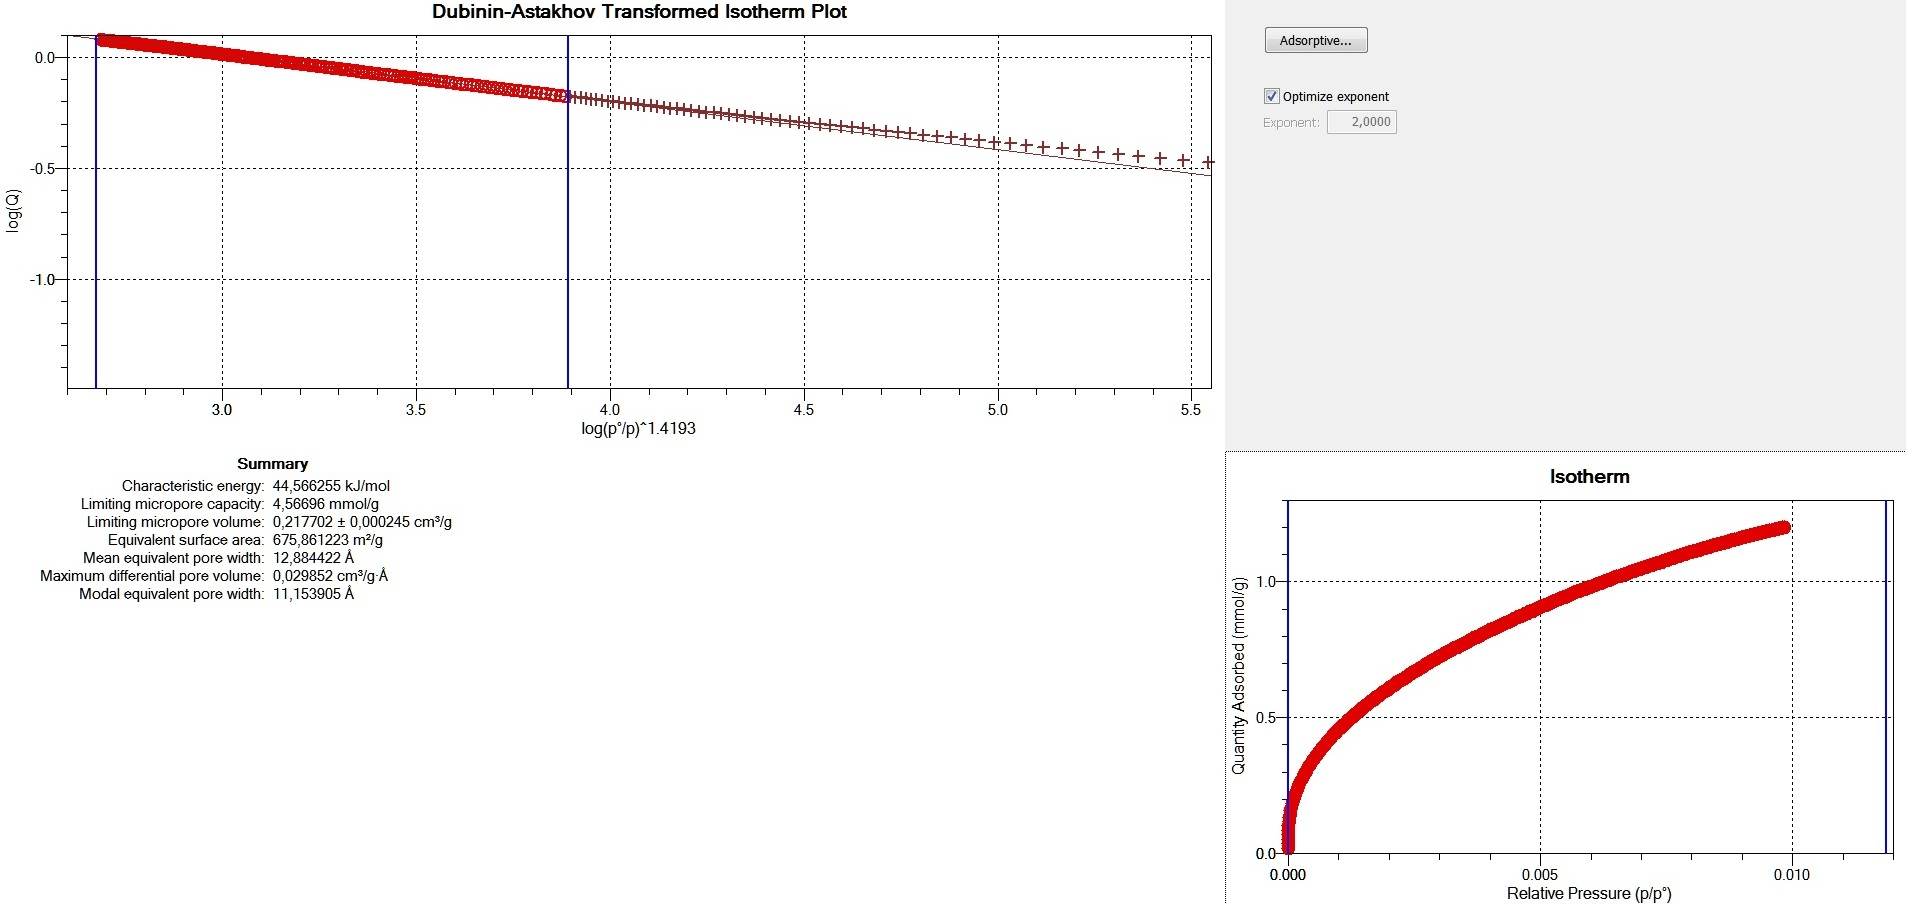
\includegraphics[height=5.2cm]{media/chem2/image104}
    \end{subfigure}
    \begin{subfigure}[t]{0.45\textwidth}
        \centering
        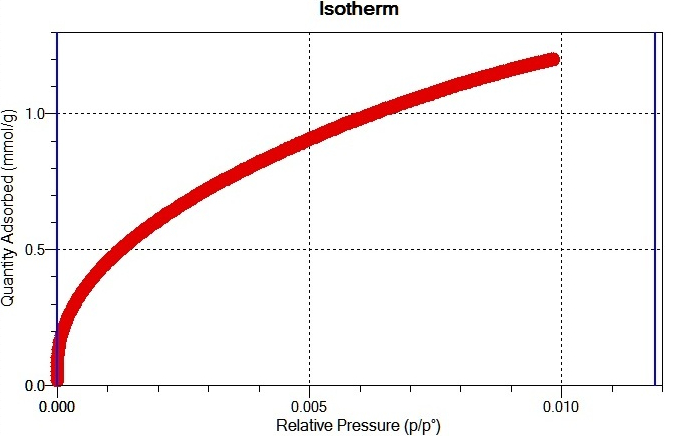
\includegraphics[height=5.2cm]{media/chem2/image104.1}
    \end{subfigure}
    \caption*{a}
    
    \begin{subfigure}[t]{0.45\textwidth}
        \centering
        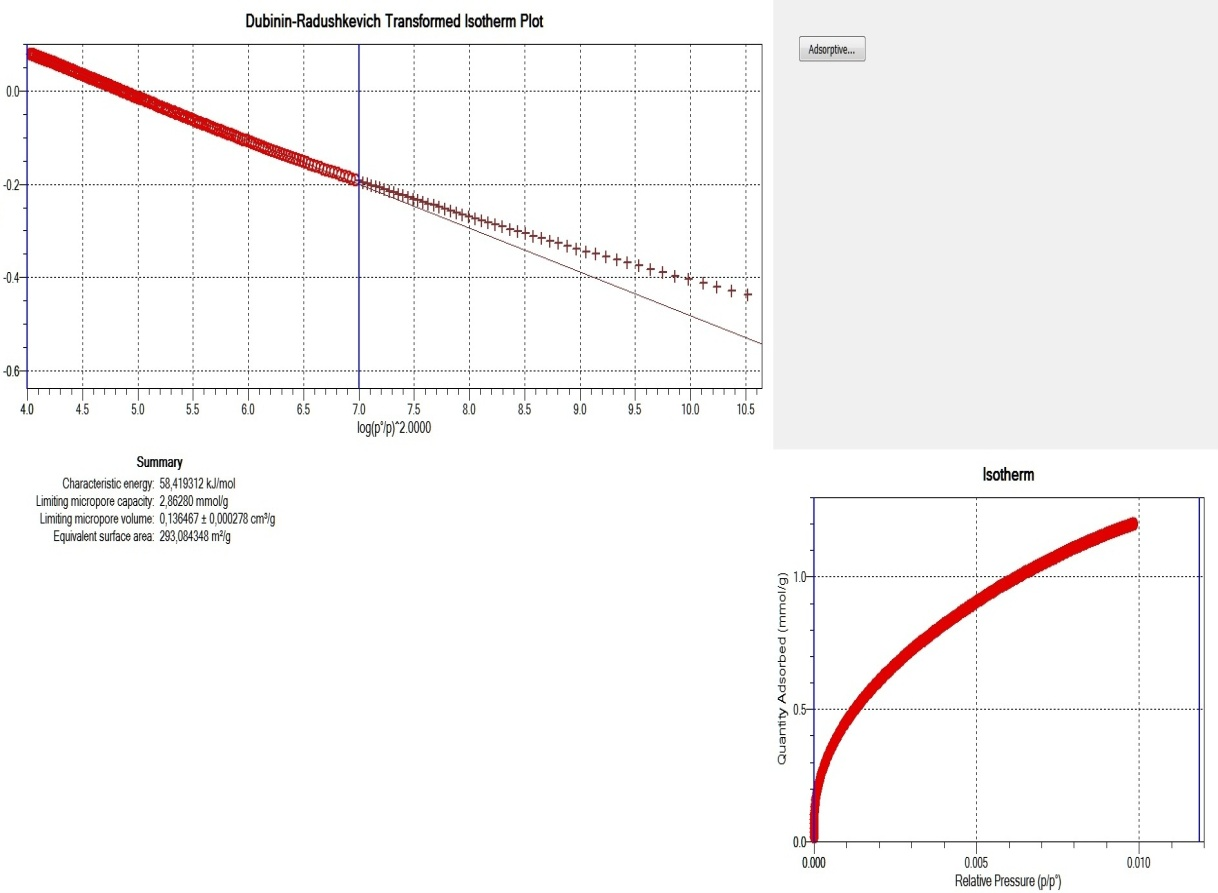
\includegraphics[height=5.2cm]{media/chem2/image105}
    \end{subfigure}
    \begin{subfigure}[t]{0.45\textwidth}
        \centering
        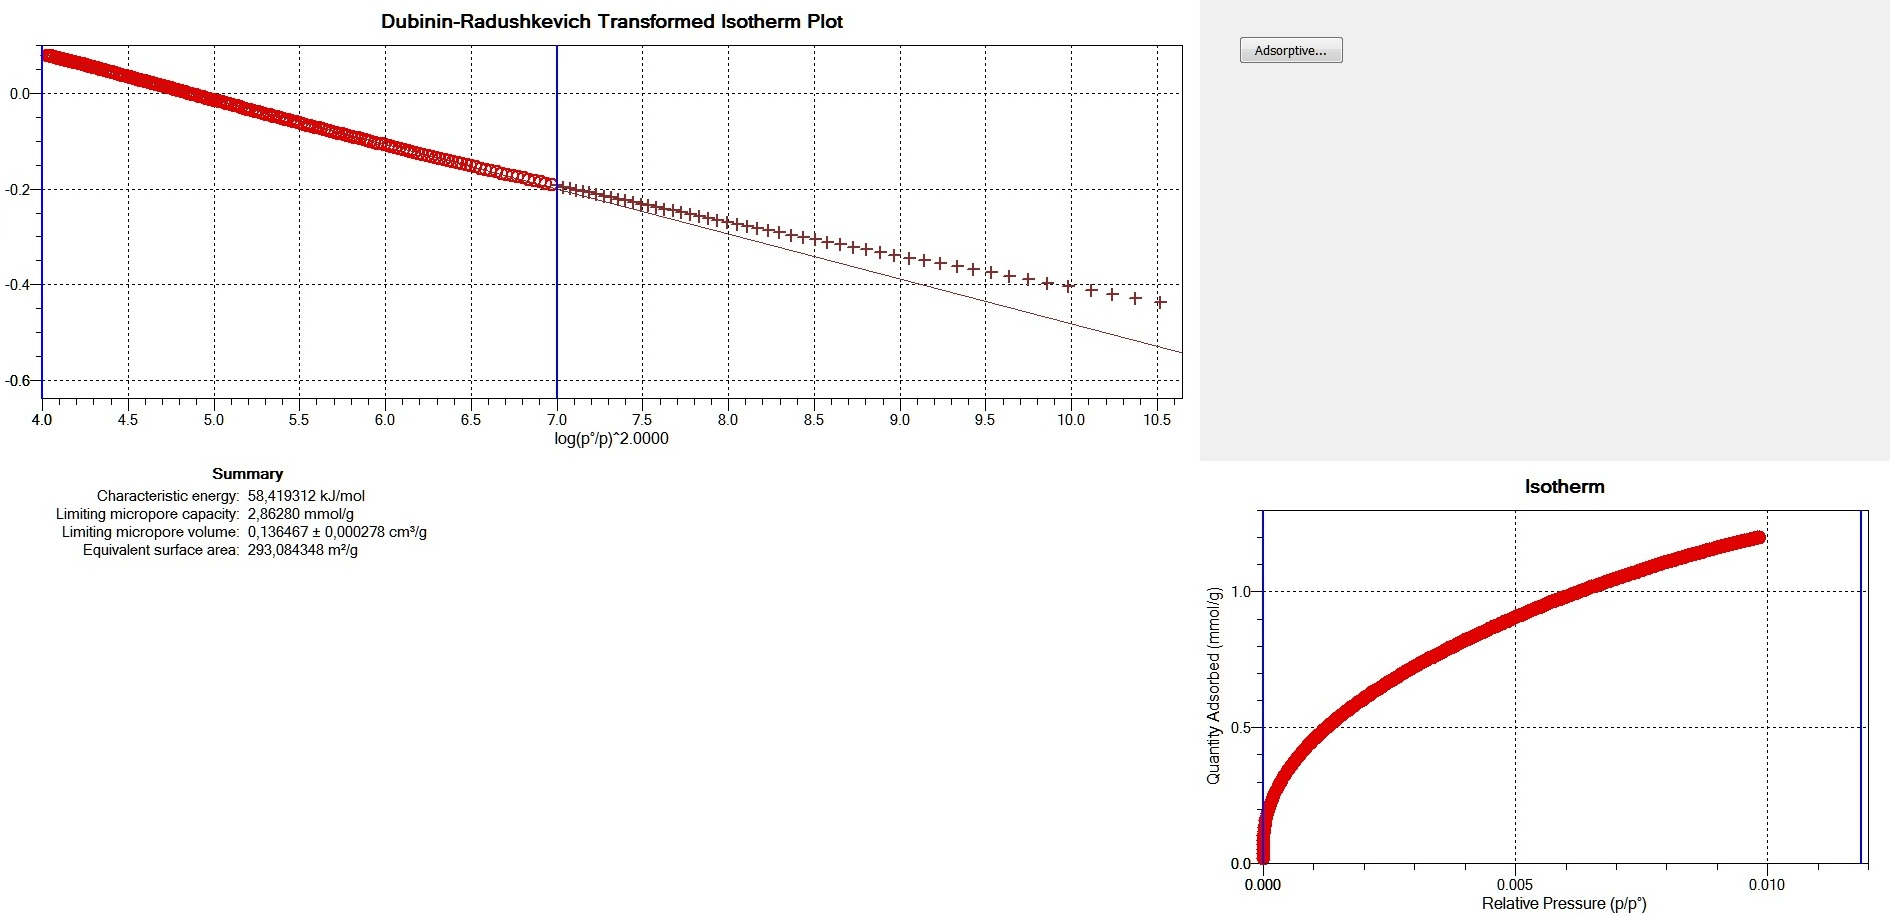
\includegraphics[height=5.2cm]{media/chem2/image106}
    \end{subfigure}
    \caption*{b}
    \caption*{Figure 5 - Adsorption curves of activated potassium humate adsorbent a-800℃, b-900℃ (according to Dubinin-Astakhov, CO\textsubscript{2})}
\end{figure}

\begin{multicols}{2}
Table 8 shows the results of calculating the porous characteristics
using the Dubinin-Radushkevich and Dubinin-Astakhov methods, showing
changes in the micropore structure of activated potassium humate with an
increase in the activation temperature.

For the sample activated at 800°C, the maximum micropore capacity using
the Dubinin-Radushkevich method is 2.8628 mmol/g, and the maximum
micropore volume is 0.136467 cm³/g. The equivalent surface area reaches
293.08 m²/g. According to the Dubinin-Astakhov method, the maximum
micropores capacity is high - 4.56696 mmol/G, and the micropores volume
limit is 0.217702 cm\textsuperscript{3} / G. when using this method, the
equivalent surface area is significantly higher and is 675.86 m2/g, and
the average equivalent pore width is 1.88 Å.
\end{multicols}

\tcap{Table 8 - Results of the study of sorption of PUM (by CO\textsubscript{2})}
\begin{longtblr}[
  label = none,
  entry = none,
]{
  width = \linewidth,
  colspec = {Q[131]Q[129]Q[121]Q[120]Q[129]Q[112]Q[100]Q[104]},
  rows = {font = \small},
  cells = {c},
  cell{1}{1} = {r=2}{},
  cell{1}{2} = {c=3}{0.35\linewidth},
  cell{1}{5} = {c=4}{0.444\linewidth},
  vlines,
  hline{1,3-5} = {-}{},
  hline{2} = {2-8}{},
}
Name & \textbf{Dubinin-Radushkevich} &  &  & \textbf{Dubinin-Astakhov} &  &  & \\
 & Maximum
			capacity of micropores, mmol/g & Maximum
			volume of micropores, cm³/g & Equivalent
			surface area, m²/g & Maximum
			capacity of micropores, mmol/g & Micropore
			volume limitation, cm³/g & Equivalent
			surface area, m²/g & Average
			equivalent pore width, Å\\
Activated
			potassium humate 800℃ & 2.8628 & 0.136467 & 293.084348 & 4.56696 & 0.217702 & 675.861223 & 1.884422\\
Activated
			potassium humate 900℃ & 2.2484 & 0.107183 & 230.192239 & 6.57723 & 0.408868 & 803.156566 & 1.303239
\end{longtblr}

\begin{figure}[H]
    \centering
    \begin{subfigure}[t]{0.45\textwidth}
        \centering
        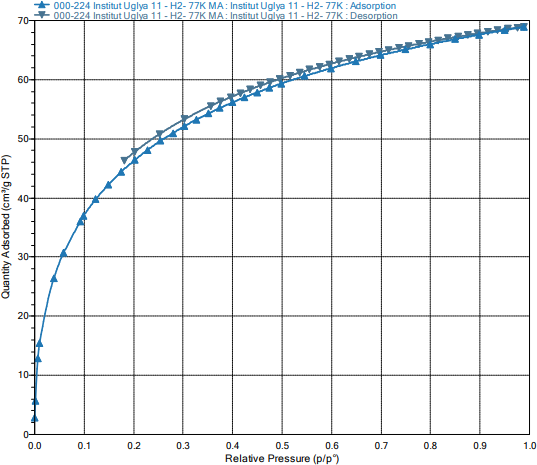
\includegraphics[width=\textwidth]{media/chem2/image107}
        \caption*{a}
    \end{subfigure}
    \begin{subfigure}[t]{0.45\textwidth}
        \centering
        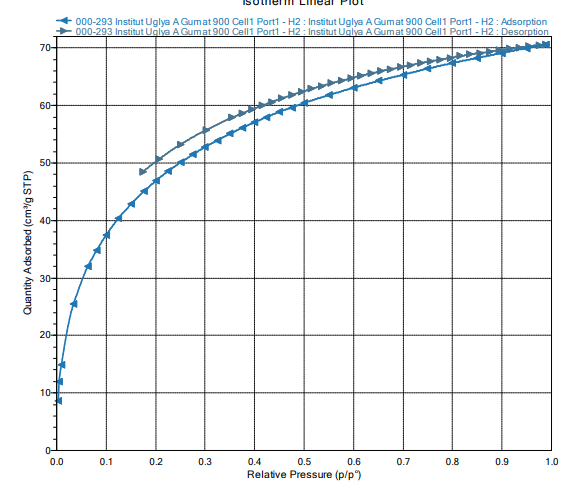
\includegraphics[width=\textwidth]{media/chem2/image108}
        \caption*{b}
    \end{subfigure}
    \caption*{Fig.6 - Adsorption curve of Activated potassium humate a-800℃, b-900℃ (H\textsubscript{2})}
\end{figure}
\vspace{-2em}
\begin{multicols}{2}
When activated at a temperature of 900°C, according to the
Dubinin-Radushkevich method, the maximum capacity of micropores
decreases to 2.24848 mmol / G, and the maximum volume of micropores
decreases to 0.107183 cm\textsuperscript{3}/g. accordingly, the
equivalent surface area decreases to 230.19 m\textsuperscript{2} / g.
however, according to the Dubinin-Astakhov method, the maximum capacity
of micropores increases to 6.57723 mmol / G, A micropores volume limit
increases to 0.408868 cm\textsuperscript{3} / G. the equivalent surface
area reaches 803.16 m\textsuperscript{2}/g, the average equivalent pore
width decreases to 1.30 Å.

A comparison of the data shows that with an increase in the activation
temperature, the volume of micropores and their equivalent width
decreases, but with the Dubinin-Astakhov method, the maximum capacity of
micropores increases. This indicates the development of a fine porous
structure, which can affect the adsorption properties of the material
and its ability to hold molecules of different sizes. The adsorption
curves of the activated adsorbent for hydrogen are shown in Figure 6.

The adsorption of hydrogen in activated potassium Humate is due to its
developed porous structure with micropores and mesopores. The main
contribution to the retention of H\textsubscript{2} is physical
adsorption on the carbon surface, which is enhanced by the presence of
narrow pores that contribute to an increase in retention forces due to
capillary condensation at low temperatures (77 K). An increase in the
activation temperature of potassium Humate leads to a slight increase in
its actual surface area and redistribution of porosity, which ultimately
contributes to an increase in hydrogen capacity.
\end{multicols}

\tcap{Table 9 - Results of the study of hydrogen sorption with potassium humate}
\begin{longtblr}[
  label = none,
  entry = none,
]{
  width = \linewidth,
  colspec = {Q[235]Q[248]Q[160]Q[294]},
  cells = {c},
  hlines,
  vlines,
}
\textbf{Name} & \textbf{Specific surface area S(\tsb{DFT}), m²/g} & \textbf{Mass of H\tsb{2}, \% (77 K)} & \textbf{Maximum amount of adsorbed H\tsb{2}, (cm}\textsuperscript{\textbf{3}}\textbf{/g)} \\
Activated potassium humate 800℃ & 130.4471 & 0.6154 & 68.9271\\
Activated potassium humate 900℃ & 130.9283 & 0.6305 & 70.6192
\end{longtblr}

\begin{multicols}{2}
The findings obtained from calculating the specific surface area and
hydrogen adsorption at a temperature of 77 kelvin suggest that the
activation of potassium humate at higher temperatures leads to a slight
improvement in sorption characteristics.

Using the DFT technique, we determined the specific surface area for a
sample that was activated at 800 degrees Celsius to be 130.4471 square
meters per gram. The mass fraction of hydrogen adsorbed at 77 degrees
Kelvin is 0.6154 percent, with a maximum amount of absorbed
H\textsubscript{2} of 68.9271 cubic centimeters per gram.

Upon increasing the activation temperature to 900 degrees Celsius, the
specific surface area marginally increases to 130.9283 square meters per
gram. Correspondingly, the mass fraction of absorbed hydrogen rises to
0.6305 percent, while the maximum amount of H\textsubscript{2}
adsorption reaches 70.6192 cubic centimeters per gram.

Consequently, despite a minor increase in the specific surface area,
activation at 900 °C leads to an enhancement in hydrogen adsorption,
which can be attributed to changes in the pore structure and the
redistribution of micropore fractions. Table 7 provides comparative
values for the calculated specific surface areas S(\textsubscript{BET})
related to the adsorption of N₂, CO₂, and H₂.

The investigation into the sorption characteristics of activated
potassium humate under a temperature of 77 K revealed a correlation
between the activation temperature and the pore structure as well as the
gas adsorption capacity of the material.

Specifically, for a sample that was activated at 800 °C, the specific
surface area was determined using the Brunauer-Emmett -Teller (BET)
method with nitrogen (N2) and amounted to 320.993 m²/g. The equivalent
specific surface area computed using the Dubinin-Radushkevich approach
with carbon dioxide (CO2) was calculated to be 293.084 m²/g, while the
Dubinin-Astakhov approach yielded a value of 675.861 m²/g. Density
functional theory (DFT) computations with hydrogen (H2) estimated the
specific surface to be 130.4471 m²/g.

Under 77 K, the amount of adsorbed hydrogen reached 0.6154\%
corresponding to a volume of 68.9271 cm³/g.

With an increase in activation temperature to 900 °C, the specific
surface area determined by the Brunauer--Emmett--Teller (BET) method
increases to 349.775 m²/g. Conversely, the equivalent specific surface
area calculated using the Dubinin--Radushkevich method decreases to
230.192 m², while the equivalent specific area determined by
Dubinin--Astakhov increases to 803.156 m².
\end{multicols}

\tcap{Table 10 -- Comparative table of specific surface area S(\textsubscript{BET}) for N\textsubscript{2}, CO\textsubscript{2} and H\textsubscript{2}}
\begin{longtblr}[
  label = none,
  entry = none,
]{
  width = \linewidth,
  colspec = {Q[92]Q[148]Q[156]Q[131]Q[233]Q[81]Q[88]},
  cells = {c},
  cell{1}{1} = {r=2}{},
  cell{1}{2} = {r=2}{},
  cell{1}{3} = {c=2}{0.287\linewidth},
  cell{1}{5} = {r=2}{},
  cell{1}{6} = {c=2}{0.168\linewidth},
  cell{3}{1} = {c=7}{0.928\linewidth},
  cell{5}{1} = {c=7}{0.928\linewidth},
  vlines,
  hline{1,3-7} = {-}{},
  hline{2} = {3-4,6-7}{},
}
\textbf{Temp\-erature, K} & \textbf{S(BET), m²/g (based on N2)} & \textbf{Equivalent specific surface area (S), m²/g (based on CO2)} &  & \textbf{Specific surface area S(DFT), m²/g (based on H2)} & \textbf{Amount of adsorbed H2 gas} & \\
 &  & \textbf{Dubinin-Radushkevich} & \textbf{Dubinin-Astakhov} &  & \textbf{\%} & \textbf{cm}\textsuperscript{\textbf{3}}\textbf{/g}\\
\textbf{Activated potassium humate (800}\textsuperscript{\textbf{0}}\textbf{С)} &  &  &  &  &  & \\
77 & 320.993 & 293.084348 & 675.861223 & 130.4471 & 0.6154 & 68.9271\\
- &  &  &  &  &  & \\
77 & 349.775 & 230.192239 & 803.156566 & 130.9283 & 0.6305 & 70.6192
\end{longtblr}

\begin{multicols}{2}
According to density functional theory (DFT), the specific surface
remains virtually unchanged at 130.9283 m². The quantity of adsorbed
hydrogen rises to 0.6305\%, or 70.6192 cm³/g.

Thus, an increase in activation temperature leads to an increase in
specific surface area and a re-distribution of porosity. This positively
affects the adsorption properties of humic substances, particularly with
regard to hydrogen adsorption. This may be attributed to alterations in
the micropore structure, resulting in an increase in narrow pores that
effectively retain hydrogen through van der Waals interactions.

{\bfseries Conclusion.} The investigation into the adsorption and
structural properties of activated potassium humate subjected to
different thermal treatments at 800°C and 900°C has shown that an
increase in the activation temperature leads to substantial alterations
in the porous structure of the material. These modifications affect the
specific surface area, the distribution of pore sizes, and the sorption
characteristics of the substance.

A comprehensive analysis of the composition reveals that at 900°C, there
is a decrease in the carbon content (from 51.06\% to 29.45\%)
accompanied by an increase in oxygen content (from 27.69\% to 31.22\%).
Additionally, there is a notable rise in the concentration of sodium and
potassium, which can be attributed to a redistribution of mineral
constituents within the structure of humate.

Raman spectroscopy analysis revealed a decline in the degree of
graphitization as the activation temperature increased, with a 27.6\%
decrease at 800°C and a 22.13\% decrease at 900°C. This was confirmed by
an increase in the intensity ratio of the D and G peaks, indicating a
rise in structural defects, which could potentially affect adsorption
properties.

The porous characteristics showed a slight increase in specific surface
area according to the Brunauer-Emmett-Teller (BET) method, from 320.99
m²/g at 800 °C to 349.77 m²/g at 900 °C, while total pore volume
remained relatively constant.

Pore structure analysis using the Dubinin--Radushkevich and
Dubinin--Astakhov models revealed changes in maximum micropore volume
and average pore size at 900 °C. Maximum micropore volume decreased,
equivalent surface area increased, and average pore diameter decreased.

The sorption characteristics of hydrogen demonstrated a slight
enhancement in the specific surface area, calculated using the DFT
method with H2, ranging from 130.45 to 130.93 square meters. The
adsorption capacity of hydrogen also increased from 0.6154\% to
0.6305\%.

This increase may be attributed to a reconfiguration of microporous
structures and the emergence of novel active sites. An increase in the
activation temperature for potassium humate resulted in an expansion of
the specific surface area and a redistribution of porosity, affecting
its adsorption capabilities. At 900°C, there was a reduction in
graphitization degree and an enhancement in hydrogen sorption capacity.
These findings indicate that humates could be employed as effective
adsorbents for hydrogen storage in gas systems.

This study confirms the promising potential of potassium humate as an
adsorbent. It opens up opportunities for the development of
cost-effective and environmentally friendly carbon-based materials for
applications in hydrogen storage, water treatment, and gas capture
technologies.

\emph{{\bfseries Acknowledgement.} This research has been funded by the
Science Committee of the Ministry of Science and Higher Education of the
Republic of Kazakhstan (Grant No. AP19577512 "Development of scientific
and technical bases for obtaining microporous carbon nanomaterials for
hydrogen separation and storage").}
\end{multicols}

\begin{center}
{\bfseries References}
\end{center}

\begin{references}
1. Satyam S., Patra S. Innovations and challenges in adsorption-based
wastewater remediation: a compre\-hensive review // Heliyon. - 2024. -
Vol.10, №.9. - P.29573. DOI 10.1016/j.heliyon.2024.e29573.

2. Chianese S. et al. Sorption of organic pollutants by humic acids: A
review //Molecules. - 2020. - Vol.25 (4). - P.918.
DOI~\href{https://doi.org/10.3390/molecules25040918}{10.3390/molecules25040918}.

3. Xie L. et al. Potassium humate-derived nitrogen-doped activated
carbons with narrow micropore size distribution for high-performance
supercapacitors //Nano. - 2017. - Vol.12 (4). - P.1750040. DOI\\
10.1142/S1793292017500400.

4. Stevenson F.J. Humus chemistry: Genesis, composition, reactions. --
2nd ed./ New York: John Wiley \& Sons. - 1994. - 512 p. - ISBN
978-0471594741

5. Lumactud R. A., Gorim L. Y., Thilakarathna M. S. Impacts of
humic-based products on the microbial community structure and
functions toward sustainable agriculture //Frontiers in Sustainable
Food Systems. - 2022. - Vol.6. - P.977121. DOI
\href{https://doi.org/10.3389/fsufs.2022.977121}{10.3389/fsufs.2022.977121}.

6. Maffia A. et al. Humic Substances: Bridging Ecology and Agriculture
for a Greener Future //Agronomy. - 2025. - Vol.15 (2). - P.410. DOI
10.3390/agronomy15020410.

7. Dzanagov S.H., Dzheliev A.S., Basiev A.E., Kanukov Z.T., Lazarov T.K.
The effect of potassium humate and micronutrients on the yield of
cucumber fruits in greenhouse conditions // BIO Web of Conferences. -
2022. - Vol.51. - Art.02002. DOI
\href{https://doi.org/10.1051/bioconf/20225102002}{10.1051/bioconf/20225102002}.

8. Benito P., Bellón J., Porcel R., Yenush L., Mulet J.M. The
biostimulant, potassium humate ameliorates abiotic stress in
Arabidopsis thaliana by increasing starch availability //
International Journal of Molecular Sciences. - 2023. - Vol.24 (15). -
Art.12140. DOI
\href{https://doi.org/10.3390/ijms241512140}{10.3390/ijms241512140}.

9. Hartmann M., Six J. Soil structure and microbiome functions in
agroecosystems // Nature Reviews Earth \& Environment. - 2022. - Vol.
4. - P.1-15. DOI
\href{http://dx.doi.org/10.1038/s43017-022-00366-w}{10.1038/s43017-022-00366-w}.

10. Zhang Z. et al. Selective modifier-assisted humic acid extraction:
Implications for soil quality enhan\-cement //Environmental Science \&
Technology. - 2024.- Vol.58 (22). - P.9896-9907. DOI\\
10.1021/acs.est.3c10713

11. Sarlaki E., Kianmehr M.H., Ghorbani M., et al. Highly humified
nitrogen-functionalized lignite activ\-ated by urea pretreatment and
ozone plasma oxidation // Chemical Engineering Journal. - 2023. - Vol.
456. - Art.140978. DOI
\href{https://doi.org/10.1016/j.cej.2022.140978}{10.1016/j.cej.2022.140978}.

12. Wang X. et al. Facile synthesis of recycling
Fe\textsubscript{3}O\textsubscript{4}/graphene adsorbents with
potassium humate for Cr (VI) removal //Colloids and Surfaces A:
Physicochemical and Engineering Aspects. - 2019. - Vol.560. - P.
384-392. DOI 10.1016/j.colsurfa.2018.10.036.

13. Kopinke F. D., Poerschmann J., Stottmeister U. Sorption of organic
pollutants on anthropogenic humic matter //Environmental Science \&
Technology. - 1995.-Vol.29 (4). - P.941-950. DOI\\
10.1021/es00004a014.

14. Puspitawati I. N. et al. Effect of Cellulose on The Characterization
of Potassium Silica--Humat Compo\-site Gel //Nusantara Science and
Technology Proceedings. - 2021. - P.57-61. DOI
10.11594/nstp.2021.1410.

15. Meng F. et al. The adsorption characteristics of uranium (VI) from
aqueous solution on leonardite and leonardite-derived humic acid: a
comparative study //Langmuir. - 2021. - Vol.37 (43). - P.
12557-12567. DOI 10.1021/acs.langmuir.1c01838.

16. Tigrine Z. et al. Sustainable Activated Carbon from Agricultural
Waste: A Study on Adsorption Effic\-iency for Humic Acid and Methyl
Orange Dyes //Sustainability. - 2024. - Vol.16 (21). - P.9308. DOI
10.3390/su16219308.

17. Janoš P. et al. Multifunctional humate-based magnetic sorbent:
Preparation, properties and sorption of Cu (II), phosphates and
selected pesticides //Reactive and functional polymers. - 2013. -Vol.
73 (1). - P.46-52. DOI
\href{https://doi.org/10.1016/j.reactfunctpolym.2012.09.001}{10.1016/j.reactfunctpolym.2012.09.001}.
\end{references}

\begin{authorinfo}
\hspace{1em}\emph{{\bfseries Information about the authors}}

Kazankapova M.K. - PhD in Philosophy, Associate Professor,
Corresponding Member of KazNANS, Leading Researcher, Head of Laboratory
of LLP "Institute of Coal Chemistry and Technology", Astana, Kazakhstan,
e-mail: maira\_1986@mail.ru;

Yermagambet B.T. -- Doctor of Chemical Sciences, Professor, Academician
of KazNANS, Project Manager, Chief Researcher, Director of LLP
"Institute of Coal Chemistry and Technology", Astana, Kazakhstan,
e-mail: bake.yer@mail.ru;

Kozhamuratova U.M. -~Junior Researcher «Institute of Coal Chemistry and
Technology», master student Eurasian National University of L.N.
Gumilyov, Astana, Kazakhstan, e-mail: kozhamuratova.u@mail.ru;

Kassenova Zh.M. - Candidate of Chemical Sciences (PhD), Associate
Professor Kazakh University of Technology and Business named after K.
Kulazhanov, Corresponding Member of KazNANS, Leading Researcher, Deputy
Director of LLP "Institute of Coal Chemistry and Technology", Astana,
Kazakhstan, e-mail: zhanar\_k\_68@mail.ru;

Malgazhdarova A.B.~-~Junior Researcher «Institute of Coal Chemistry and
Technology», master student Eurasian National University of L.N.
Gumilyov, Astana, Kazakhstan, e-mail: malgazhdarova.ab@mail.ru;

Dauletzhanova Zh. T.~- PhD~Doctor, Technology, Kazakh University of
Technology and Business named after K. Kulazhanov, Leading Researcher
of~ LLP "Institute of Coal Chemistry and Technology"~Astana,
Kazakhstan, e-mail: \\kaliyeva\_zhanna@mail.ru;

Cygan A. - Leading Researcher Institute Of Technology And Fuel
Processing Technology, Zamkowa 1, 41-803 Zabrze, Poland,
e-mail: acygan@itpe.pl;

Mendaliyev G. K. -~Junior Researcher «Institute of Coal Chemistry and
Technology», master student Eurasian National \\University of L.N.
Gumilyov, Astana, Kazakhstan, e-mail: ganimen02@mail.ru;

Akshekina A.S. -~Senior Lab Assistant «Institute of Coal Chemistry and
Technology», master student Eurasian National \\University of L.N.
Gumilyov, Astana, Kazakhstan, e-mail: akshekina11@gmail.com;

Tarikhov F. - Research technologist, Nazarbayev University, Astana,
Kazakhstan, e-mail: farkhad.tarikhov@nu.edu.kz

\hspace{1em}\emph{{\bfseries Сведения об авторах}}

Казанкапова М.К. -PhD, асс. профессор, чл.-корр. КазНАЕН,
ведущий научный сотрудник, заведующий лабораторией ТОО «Институт химии и
технологии угля», Астана, Казахстан, e-mail: maira\_1986@mail.ru;

Ермагамбет Б.Т. - доктор химических наук, профессор, академик КазНАЕН,
руководитель проекта, главный научный сотрудник, директор ТОО «Институт
химии и технологии угля», Астана, Казахстан,  e-mail: bake.yer@mail.ru;

Қожамұратова Ұ.М. - младший научный сотрудник ТОО «Институт химии угля и
технологии», магистрант Евразийского национального университета им.
Л.Н.Гумилева, Астана, Казахстан, e-mail: kozhamuratova.u@mail.ru;

Касенова Ж.М. -- кандидат химических наук (PhD), и.о асс. профессор
Казахского университета технологии и бизнеса имени К. Кулажанова,
чл.-корр. КазНАЕН заместитель директора ТОО «Институт химии и технологии
угля», Астана, Казахстан, e-mail: zhanar\_k\_68@mail.ru;

Малғаждарова А.Б. -- младший научный сотрудник ТОО «Институт химии угля
и технологии», магистрант Евразийского национального университета им.
Л.Н.Гумилева, Астана, Казахстан, e-mail: malgazhdarova.ab@mail.ru;

Даулетжанова Ж.Т. - доктор PhD, доцент Казахского университета
технологии и бизнеса имени К. Кулажанова, Астана, ведущий научный
сотрудник ТОО «Институт Химии угля и технологии», Астана, Казахстан
e-mail: \\kaliyeva\_zhanna@mail.ru;

Цыган А. - ведущий научный сотрудник Институт технологии и переработки
топлива, Замкова 1, 41-803 Забже, Польша, e-mail: acygan@itpe.pl;

Мендалиев Г.К. - младший научный сотрудник ТОО «Институт химии угля и
технологии», магистрант Евразийского национального университета им.
Л.Н.Гумилева, Астана, Казахстан, e-mail: ganimen02@mail.ru

Акшекина Ә.С. -  старший лаборант ТОО «Институт химии угля и
технологии», Астана, Казахстан, e-mail: \\akshekina11@gmail.com;

Тарихов Ф. - научный технолог в Офисе коллективного пользования при
Назарбаев Университете, Астана, Казахстан, e-mail: farkhad.tarikhov@nu.edu.kz
\end{authorinfo}
